\documentclass[11pt,letter]{article}
\usepackage[top=1.00in, bottom=1.0in, left=1.1in, right=1.1in]{geometry}
\renewcommand{\baselinestretch}{1.1}
\usepackage{graphicx}
\usepackage{natbib}
\usepackage{amsmath}

\def\labelitemi{--}
\parindent=0pt

\begin{document}
\bibliographystyle{/Users/Lizzie/Documents/EndnoteRelated/Bibtex/styles/besjournals}
\renewcommand{\refname}{\CHead{}}

\title{Temporal Ecology Lab guide to\\ forest tree demography} 
\author{E M Wolkovich} 
\date{\today}
\maketitle

\emph{So far these notes are all based on what Lizzie learned from visiting Janneke Hille Ris Lambers setup on Mount Rainier in June 2020.}
\section{Adult trees}

For adult trees you basically need big plots where you map (location) every tree with a $>$5 cm DBH (I think that's the size, should check). Ideally you tag everything, take DBH and height, and revisit the plots to keep measuring the trees (Janneke uses a system of plots already set up, that is revisited every 5 years for a re-census).

\section{Germinants and seedlings}

This is what I wanted to learn about! Janneke counts all germinants (aka 1-year-old seedlings, which I found confusing because they are only a couple months old at most, but whatever) to species (ID notes below) in a 1 $m^2$ plot each year, but does NOT tag any. She tags all 2-year-old seedlings (or older) with cute cocktail-style toothpicks (see Fig. \ref{fig:tagged}-\ref{fig:tshe}). She had sturdier picks than I could find, but she had a good diversity so all could be tagged uniquely (for each marked seedling, she recorded the approximate coordinates within the plot of seedling and the tag, for example `blue club' or `red sword') and measures their height and presence each year. So a normal plot would include: (1) count all the germinants to species, (2) check all the previously recorded seedlings for height and presence and (3) tag (and record details) of any new 2-year-old seedlings.\\

\emph{Telling apart 1- and 2-year-old seedlings can be hard}, especially if the 2-year-old seedlings have not put on true (non-cotyledon) leaves (note that 1-year-old seedlings can go for it and have true leaves the first year, even within a month or such). Things to look for are any sign of woodiness in the stem and whether the cotyledons show signs they have been through a season of wear and tear. \\

{\bf ID info:} The most common one we saw were THSE (hemlock) and THPL (cedar); these are smaller and about the same size, the THPL has 2 cotyledons, while the THSE has usally 3-4 cotyledons. Two-year-old THPL look a lot like moss but then eventually go all `Frankenstein' and shoot out a cedar-looking leaf. \emph{Abies} germinants can have drunken looking cotyledons (curled etc.) and are larger than THSE and THPL. PSME (Doug Fir) is also larger but will not have any drunken-looking cotyledons; it will have POINTY ends (see Figs. \ref{fig:seedling}, \ref{fig:PSMEup}, \ref{fig:PSMEreg}, \ref{fig:PSMEmunched}). \\

{\bf Guides:} Janneke first sent ``Kaiser\_PNW\_SeedlingGuide\_2019.pdf'' and later (July 2020) sent ``MORA seedling pics.pdf'' which is similar to what I saw them use in the field (``GerminantIDbooklet.pdf'', which should have a lot of overlap with ``MORA seedling pics.pdf''  but has some nice features, like a table for quick ID). 

\section{Seeds}

Janneke also monitors seeds using seed traps (which look a lot like litter traps to me, notes on construction below). She collects them once a year in the spring when doing germinant counts etc.---you scrape out all the contents (if there are cones or small twigs or moss or basically anything on top that could be hiding seeds, also include all that too) into a paper bag (which you keep in a plastic bag because they can get wet). Bring home all the contents, sort out the seeds, dry, count.

\section{Plot setup, equipment etc.}
Overall setup was 6 plot units (including a litter trap and a 1 $m^2$ plot where they measured percent cover---categories: bare/litter/nurselog/moss/veg), canopy cover (densiometer), soil moisture (four random spots) and counted all germinants and kept track of all seedlings (see Fig. \ref{fig:plot}). The plots were set at the same transect line in each bigger forest tree plot and were equidistant from one another. Janneke was debating whether it would be better to do three 0.5 x 0.5 $m$ plots instead of the big 1 $m^2$ one. She may change her design for any new plots she sets up in Europe.\\

Seed trap construction (see Fig. \ref{fig:seedtrap}): These were rectangular laundry baskets with holes drilled in the bottom to let out water. You need to make fine mesh liners (make sure the seams face OUT---towards the basket, not towards the part of the liner you will be scraping and trying to scoup seeds and debris out of) that fit in the baskets, and then put chicken wire on top to prevent too much debris getting in. Put the wire on top and use binder clips on two sides to keep the chicken wire in place. The traps were firmly rooted on the group via 10 inch tent stakes (attached to the baskets with wire). \\

Janneke uses a $\delta T$ (DeltaT) Soil Moisture Kit (SM150) which she liked for measuring soil moisture for germinants and seedlings since it's a shallow soil depth probe. 


\begin{figure}[h!]
\centering
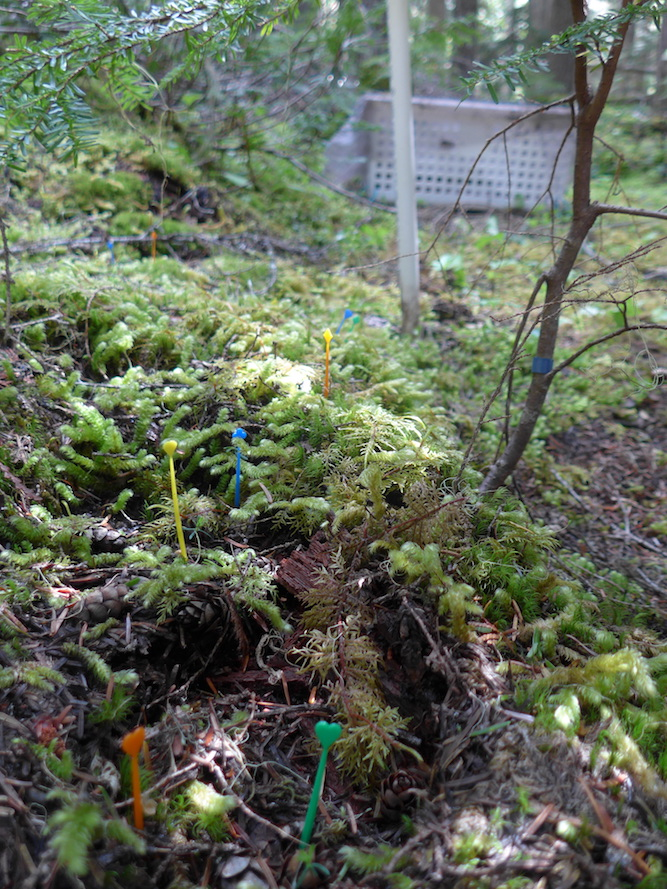
\includegraphics[width=0.95\textwidth]{images/2020June18_Rainier237sm.jpg}
\caption{A field of tagged germinants, with a seed trap in the distance.}
\label{fig:tagged} 
\end{figure}

\begin{figure}[h!]
\centering
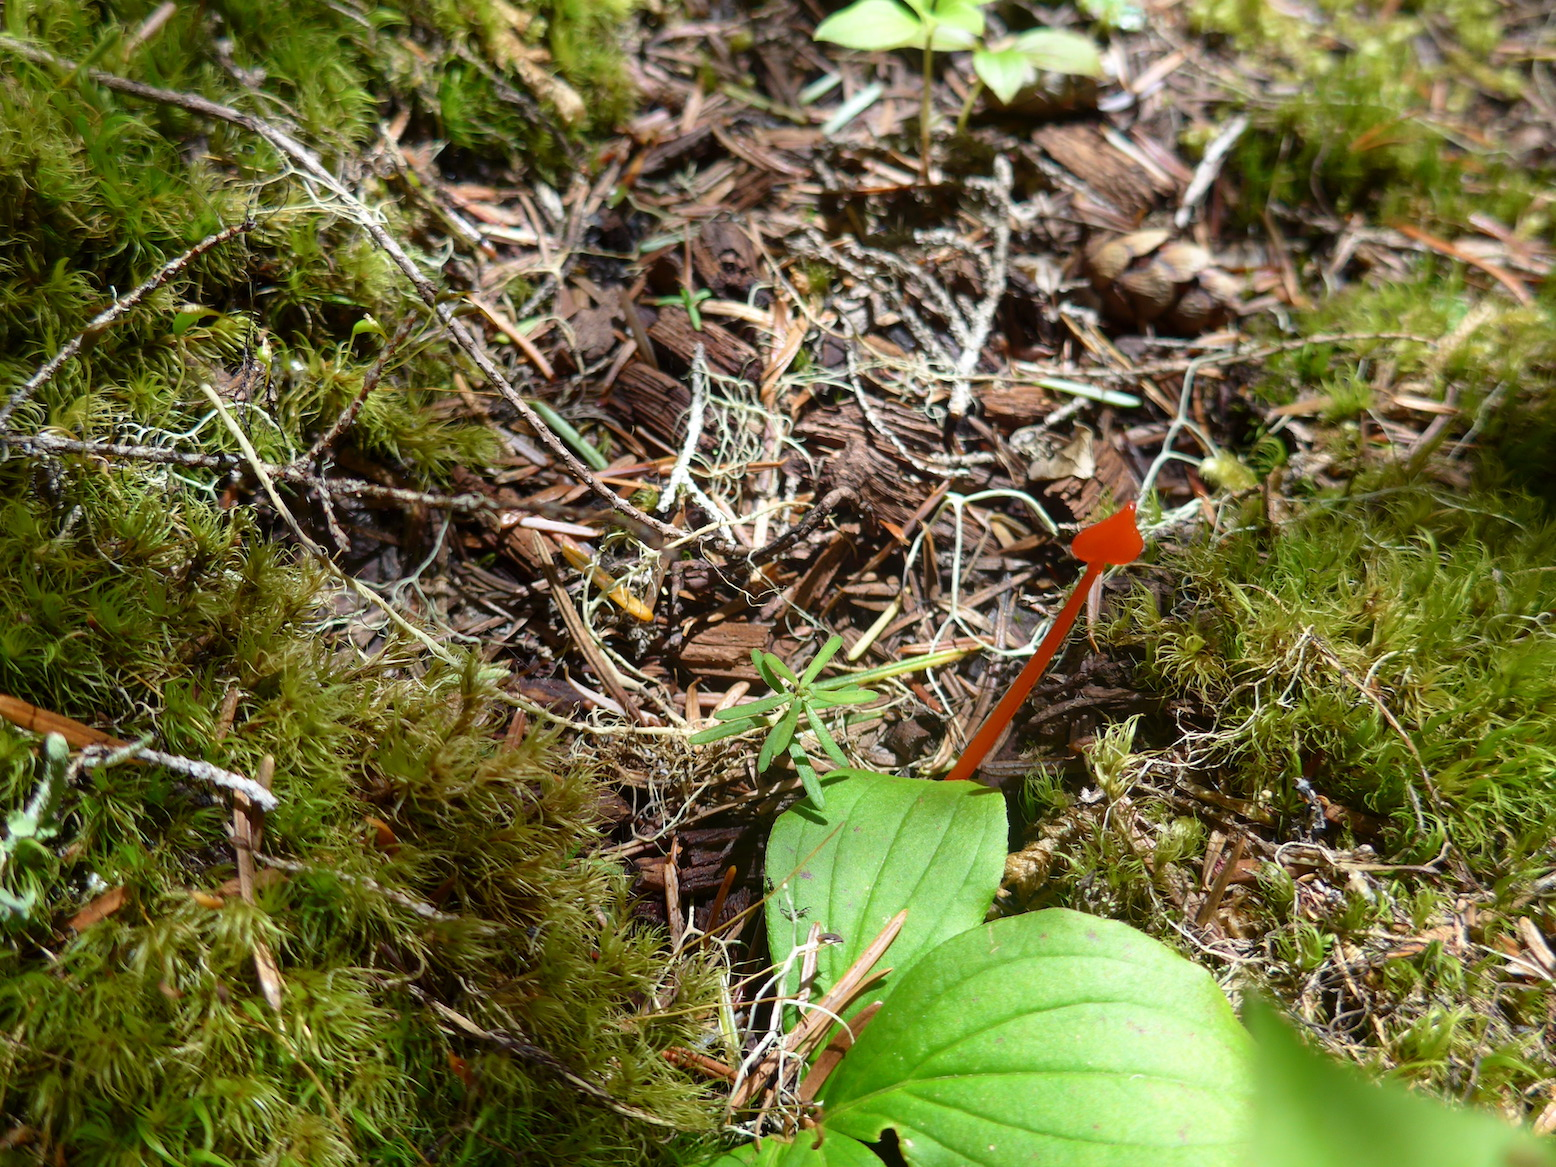
\includegraphics[width=0.95\textwidth]{images/2020June18_Rainier247smTSHE.jpg}
\caption{A tagged TSHE seedling.}
\label{fig:tshe} 
\end{figure}



\begin{figure}[h!]
\centering
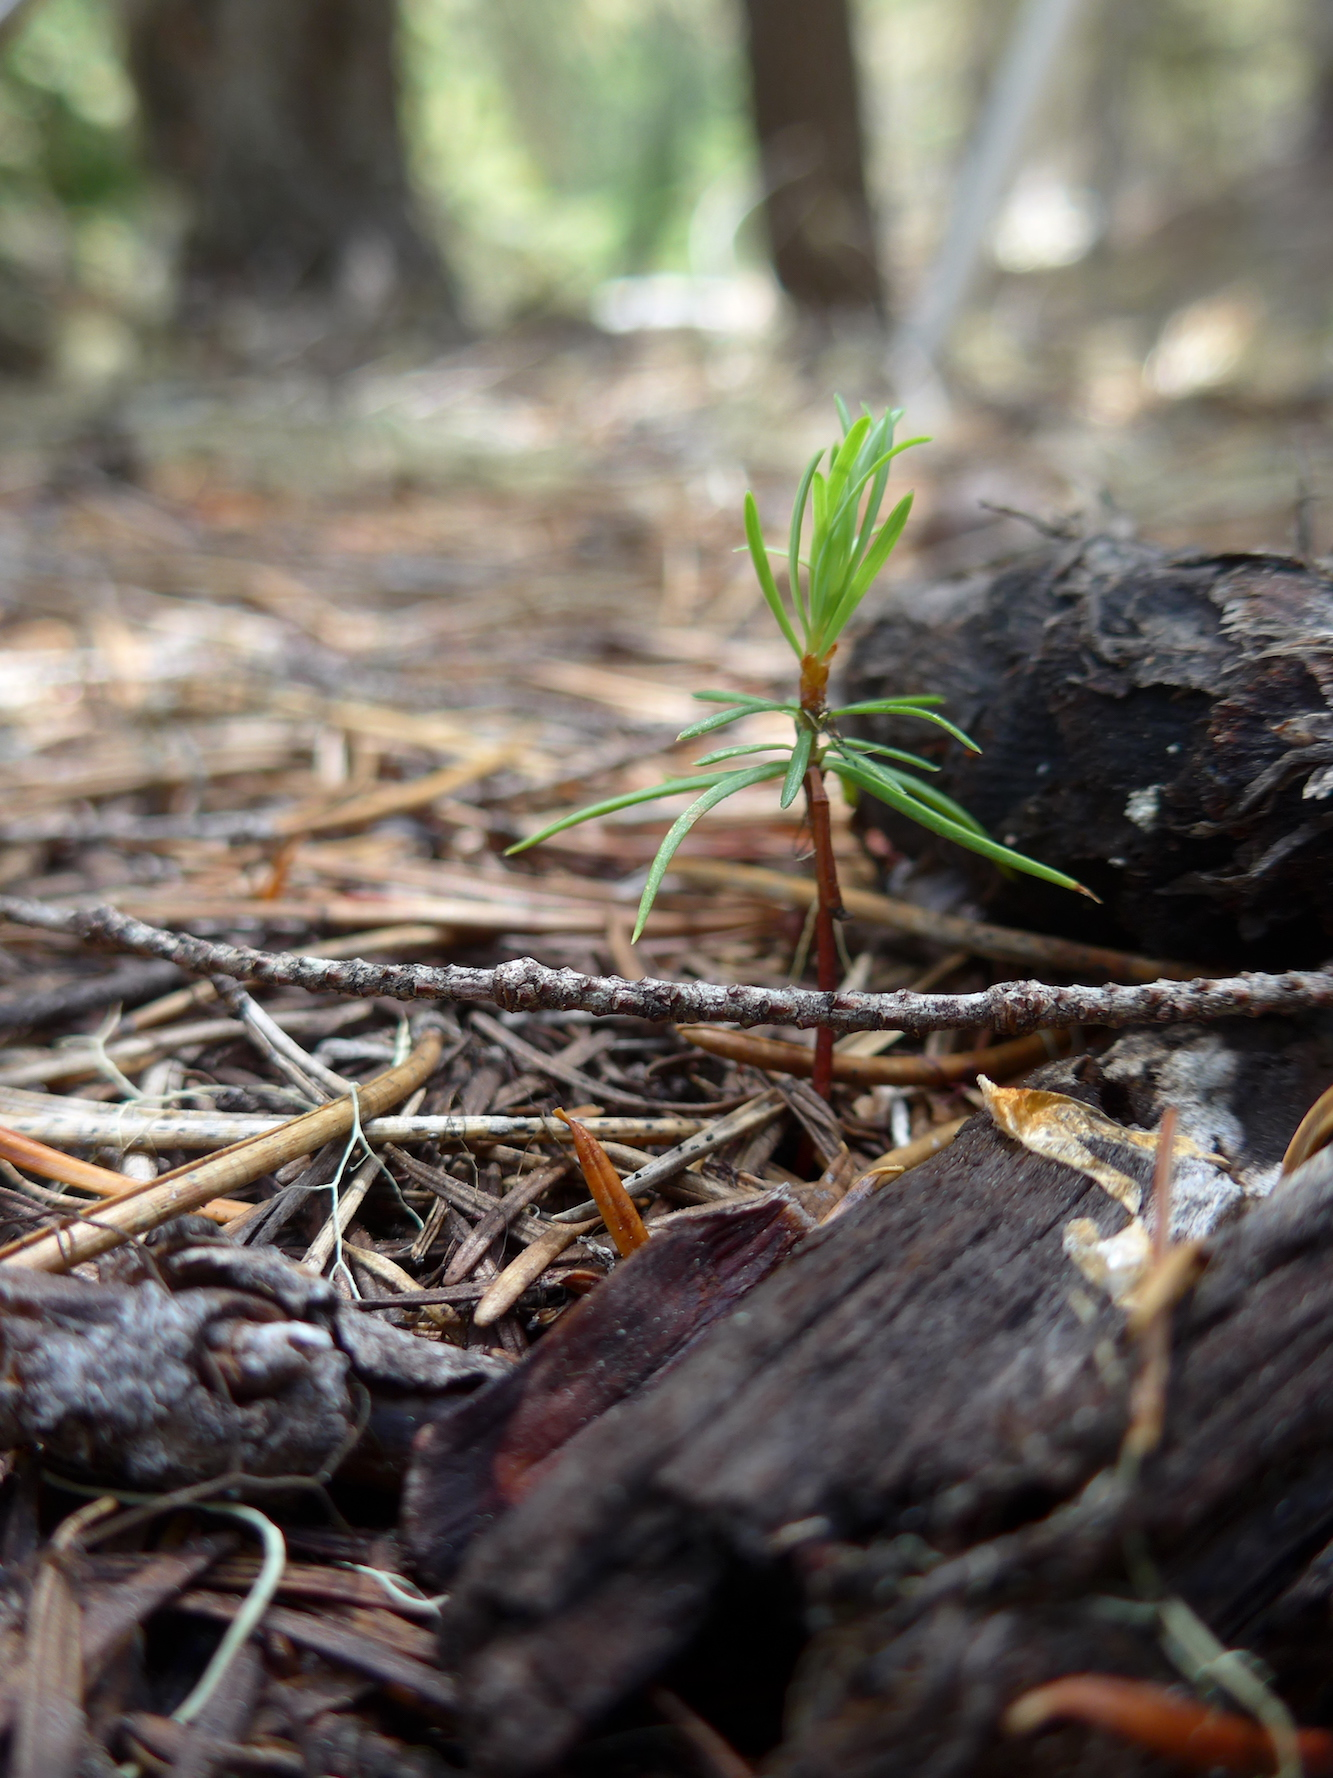
\includegraphics[width=0.95\textwidth]{images/2020June17_Rainier206sm.jpg}
\caption{PSME or PICO older seedling.}
\label{fig:seedling} 
\end{figure}


\begin{figure}[h!]
\centering
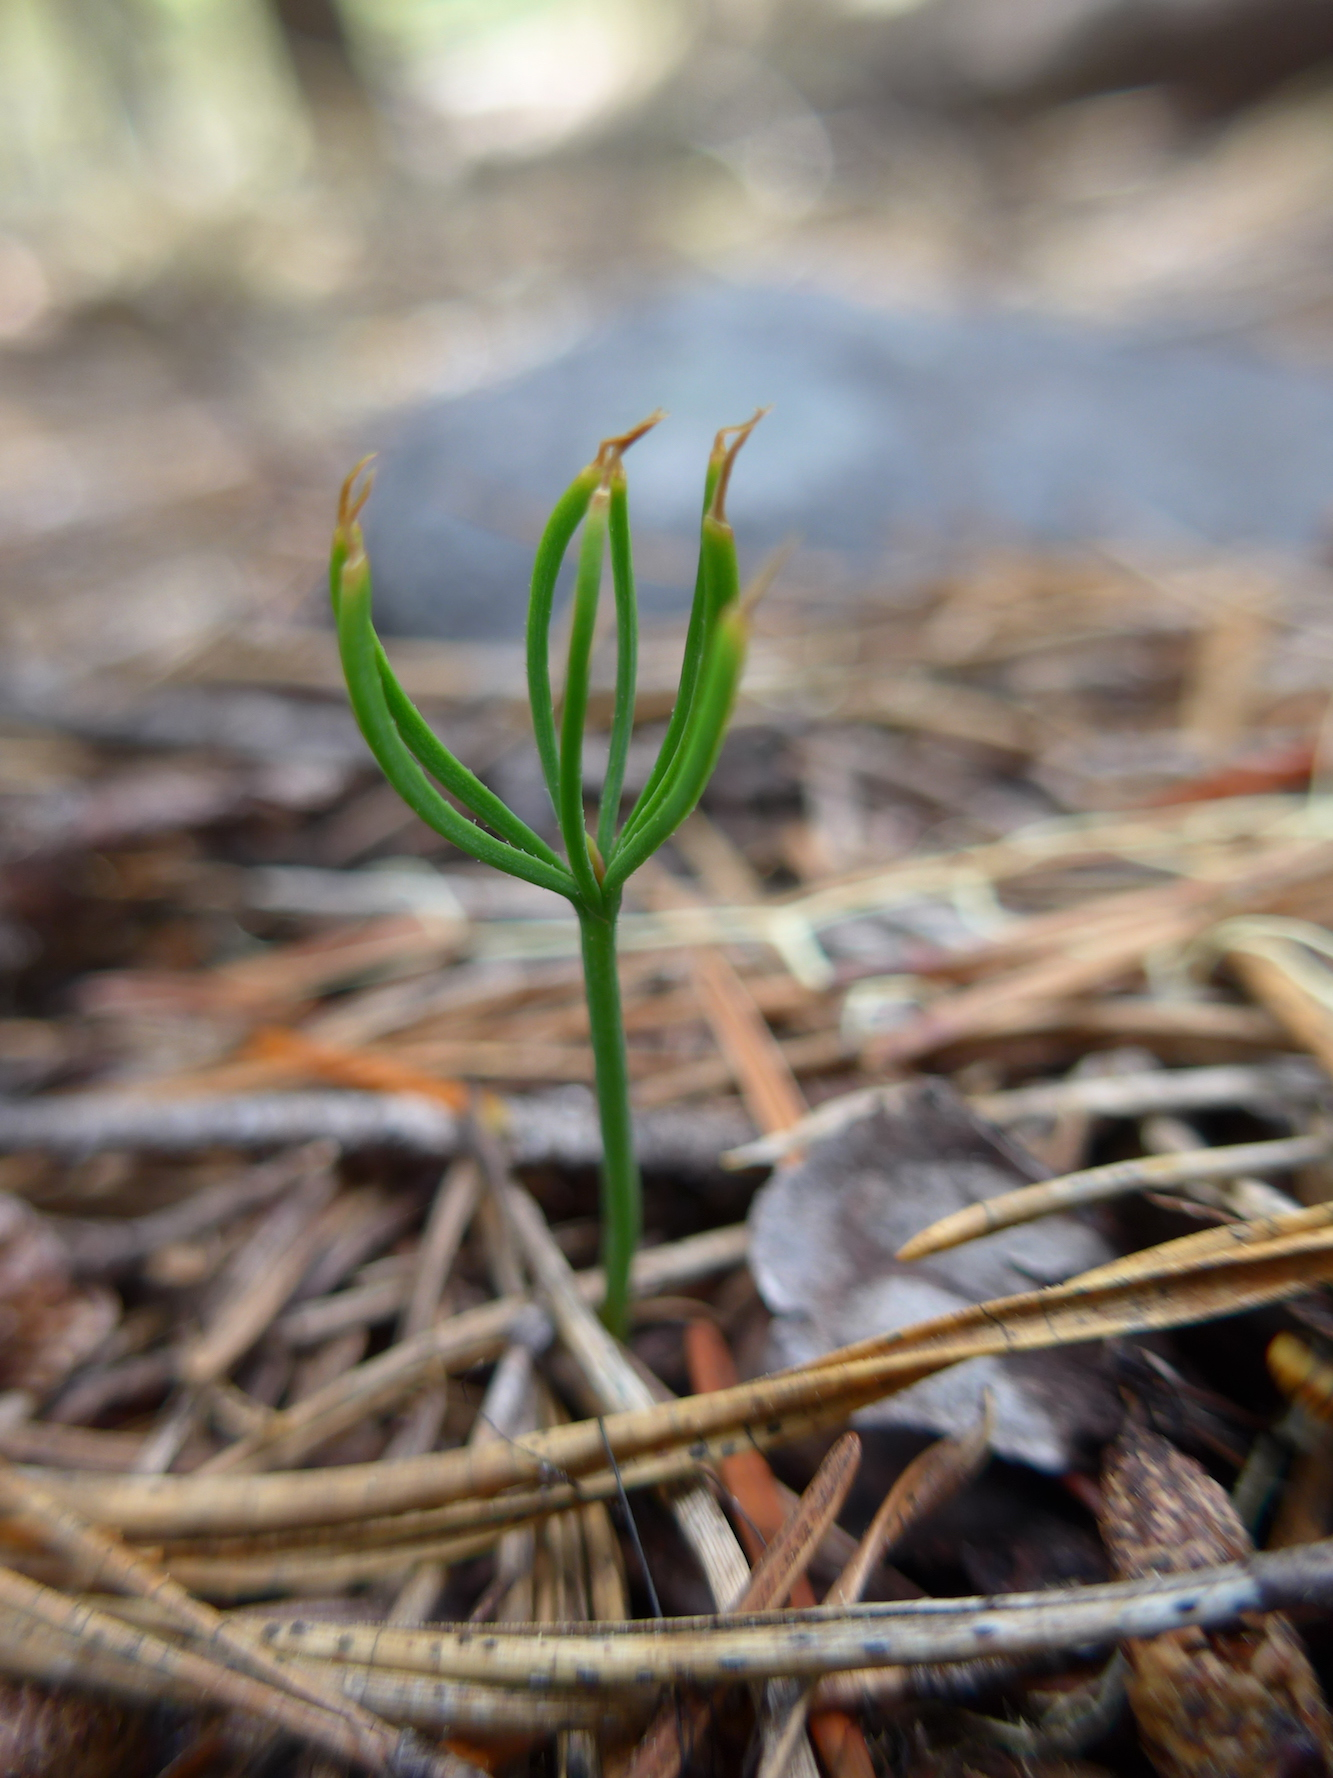
\includegraphics[width=0.95\textwidth]{images/2020June17_Rainier209_PSMEsm.jpg}
\caption{PSME germinant, not yet having let its cotyledons down.}
\label{fig:PSMEup} 
\end{figure}

\begin{figure}[h!]
\centering
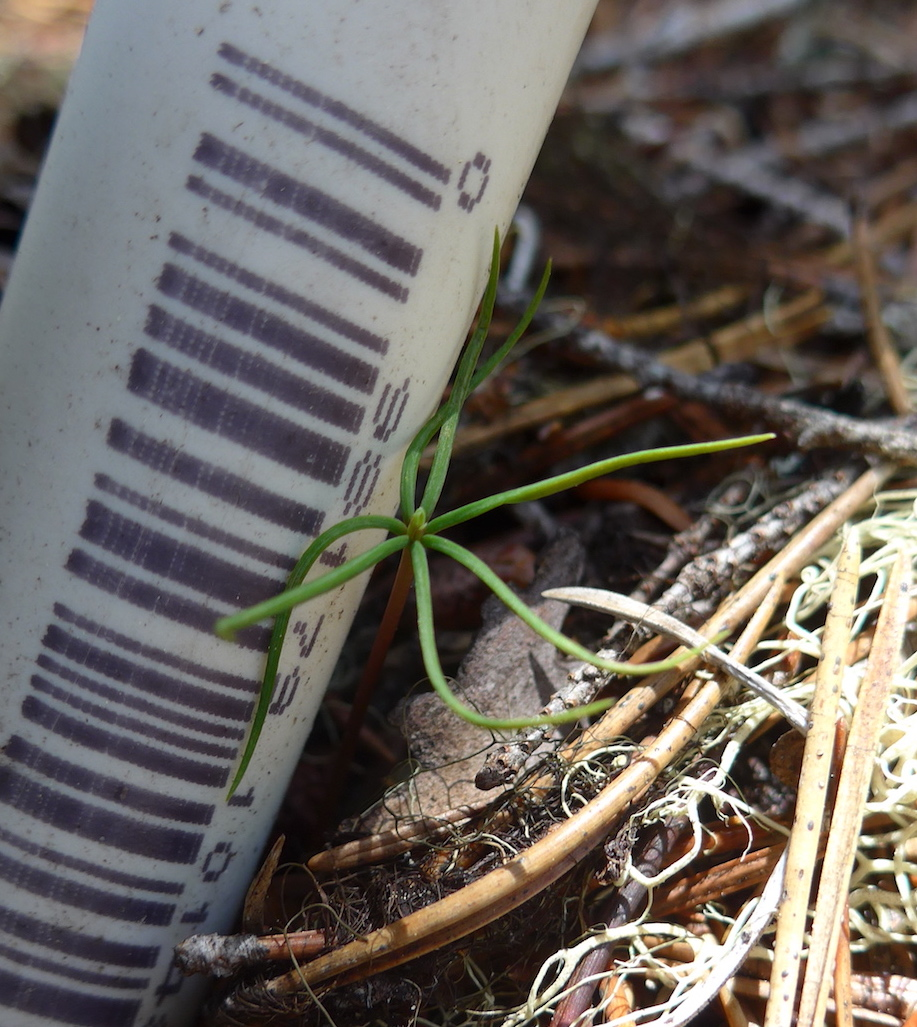
\includegraphics[width=0.95\textwidth]{images/2020June17_Rainier210PSMEsm.jpg}
\caption{PSME germinant, looking more regular (though smushed against a pole).}
\label{fig:PSMEreg} 
\end{figure}


\begin{figure}[h!]
\centering
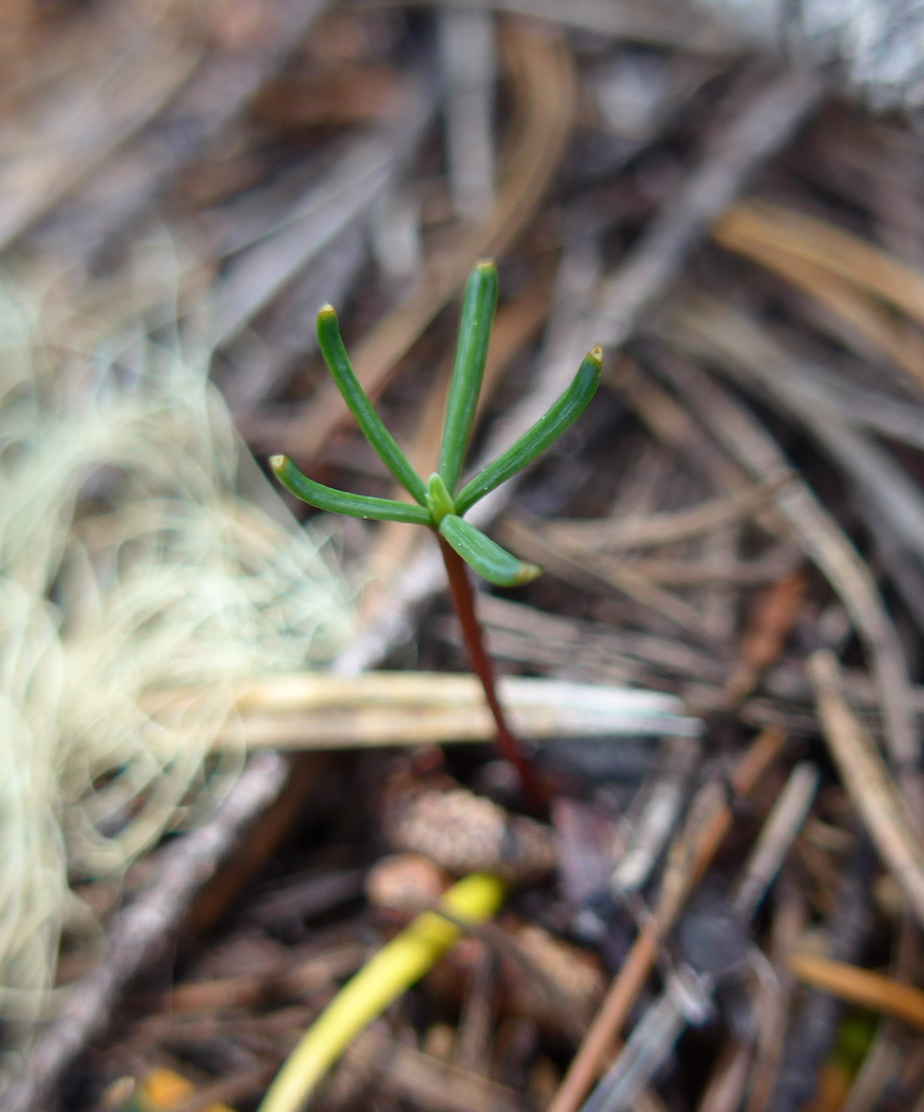
\includegraphics[width=0.95\textwidth]{images/2020June17_Rainier203_munchedPSMEsm.jpg}
\caption{PSME germinant with munched cotyledons.}
\label{fig:PSMEmunched} 
\end{figure}



\begin{figure}[h!]
\centering
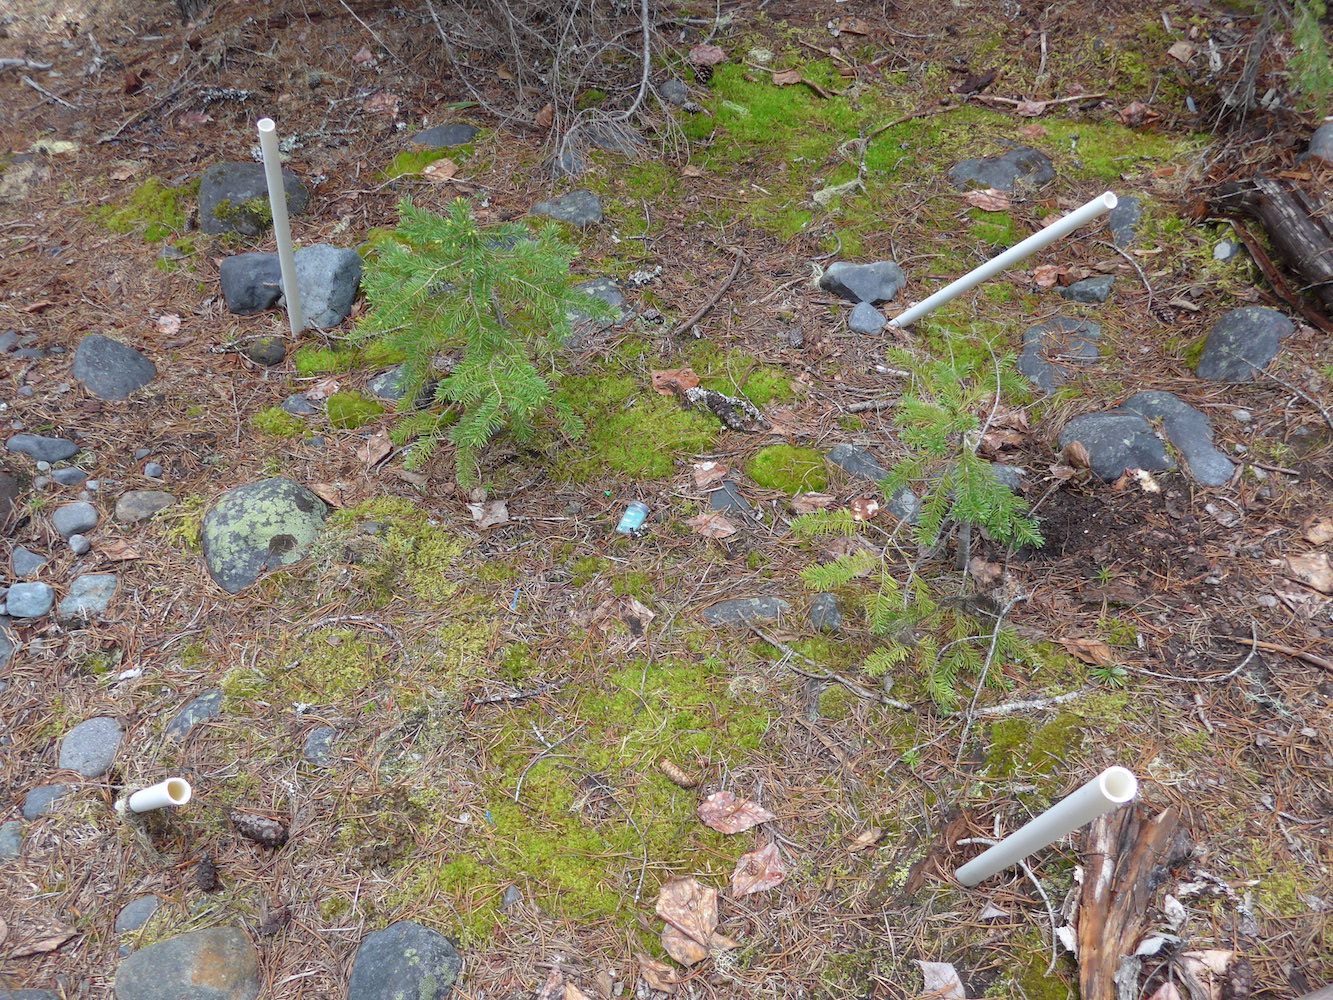
\includegraphics[width=0.95\textwidth]{images/2020June17_Rainier188sm.jpg}
\caption{A 1 m x 1m plot for monitoring germinants (Hobo data logger in the middle).}
\label{fig:plot} 
\end{figure}


\begin{figure}[h!]
\centering
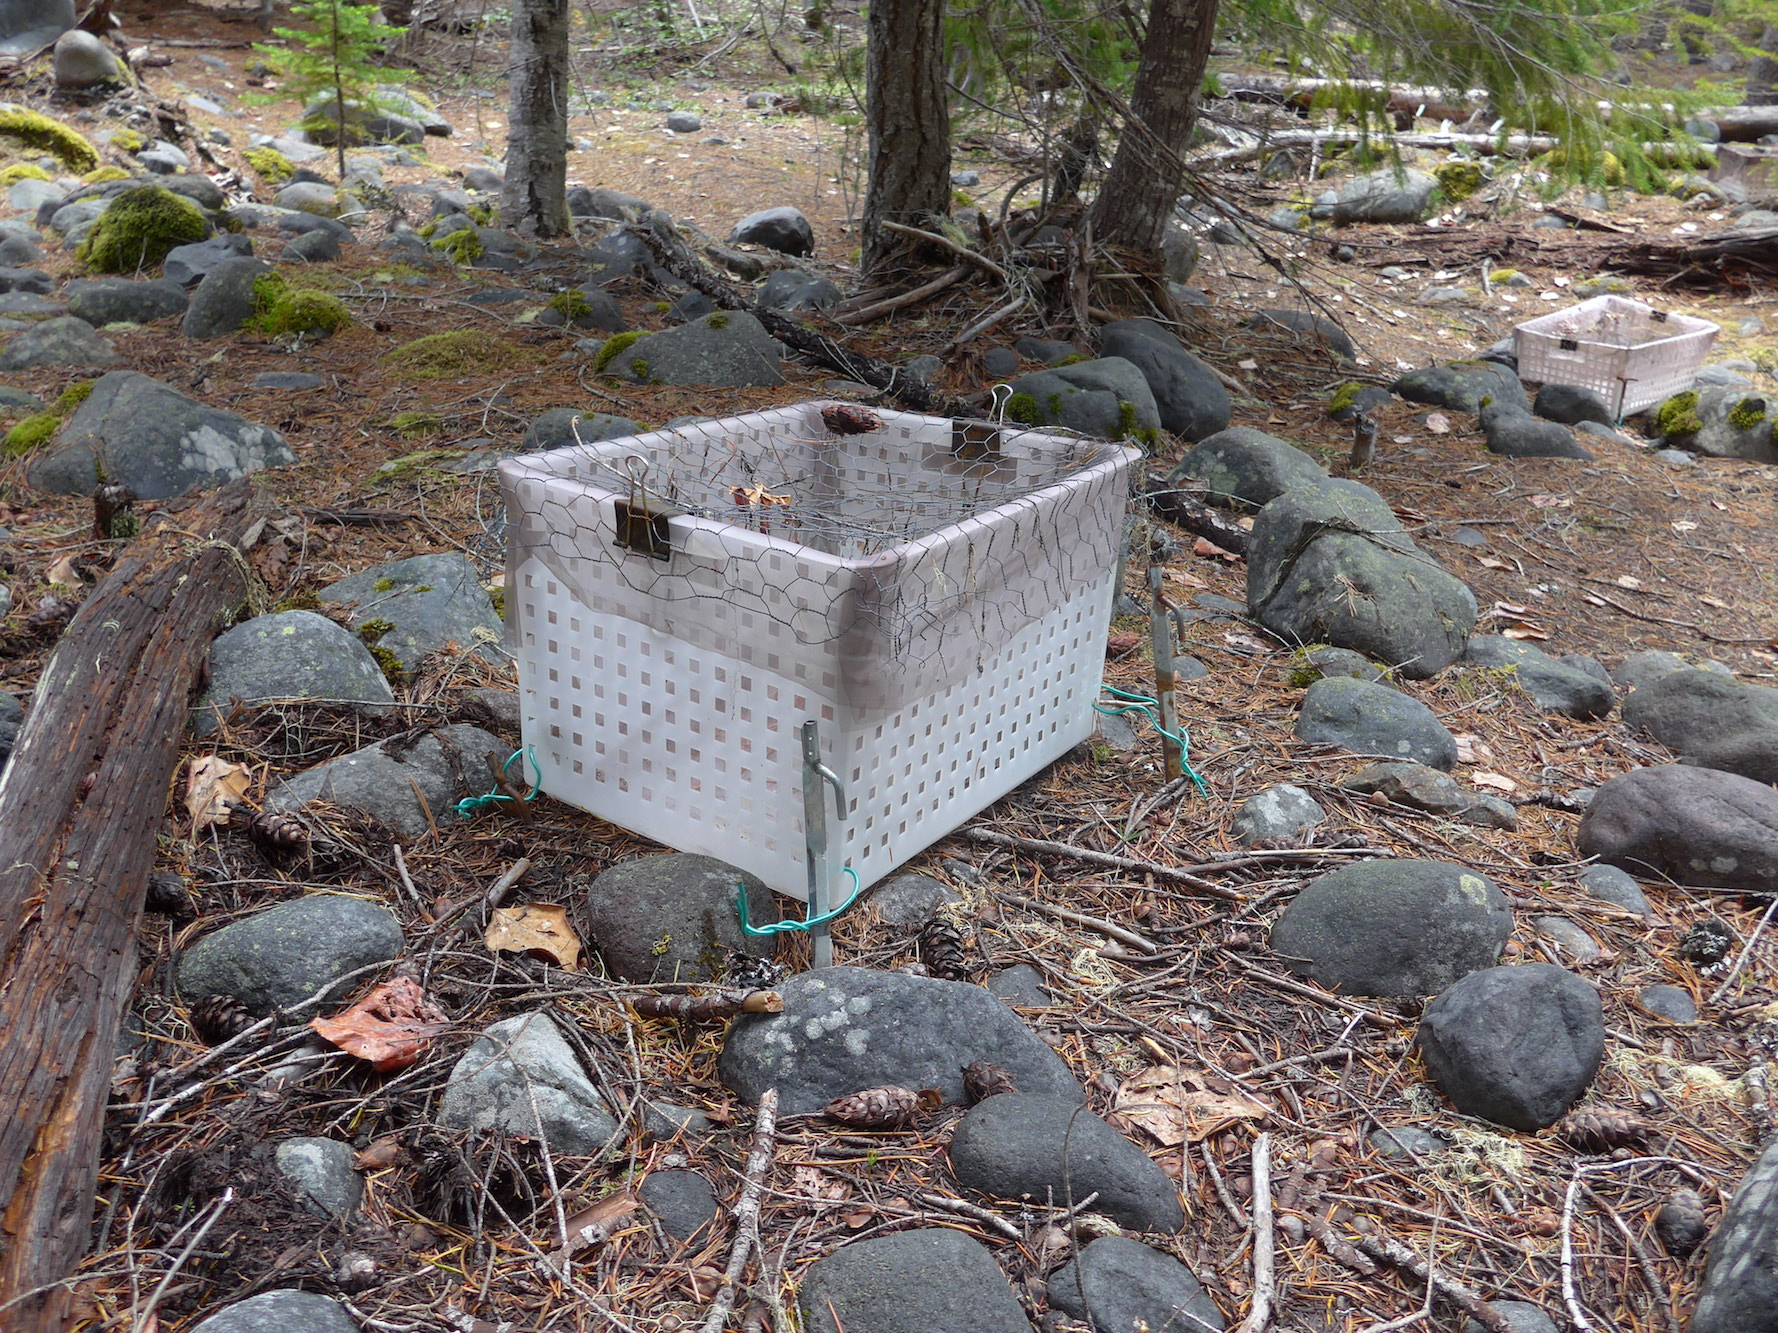
\includegraphics[width=0.95\textwidth]{images/2020June17_Rainier185sm.jpg}
\caption{A seed trap, the tent stakes are shown only because they ground was too rocky to fully sink them.}
\label{fig:seedtrap} 
\end{figure}


\end{document}